\chapter{相关技术概述}
\section{WireShark网络分析工具}
WireShark是开源网络包分析工具。主要作用是能够在网卡接口处捕获数据包,并显示数据包中的具体协议信息\cite{wireshark1}。其适用于Windows和UNIX系统,且支持多协议的网络数据包解析。
在实践过程中,网络管理员用其检测网络波动问题,网络安全工程师用它来检查安全相关问题,协议开发者则使用它来测试新的通讯协议\cite{wireshark2}。
本文中使用Wireshark对进口FFS中的仿真机发送的数据包进行捕获,为是研究其使用的通信协议,进而将自主研发的视景系统接入该仿真机中。
\par
数据包捕获界面如图\ref{wireshark}所示,上方是捕获到的所有数据帧列表;左下方是所选数据帧的信息分析,包括其使用的网络协议、长度信息等;
右下方则是这个数据帧的具体内容,以十六进制的形式展现。
\begin{figure}[h!]
    \begin{center}
        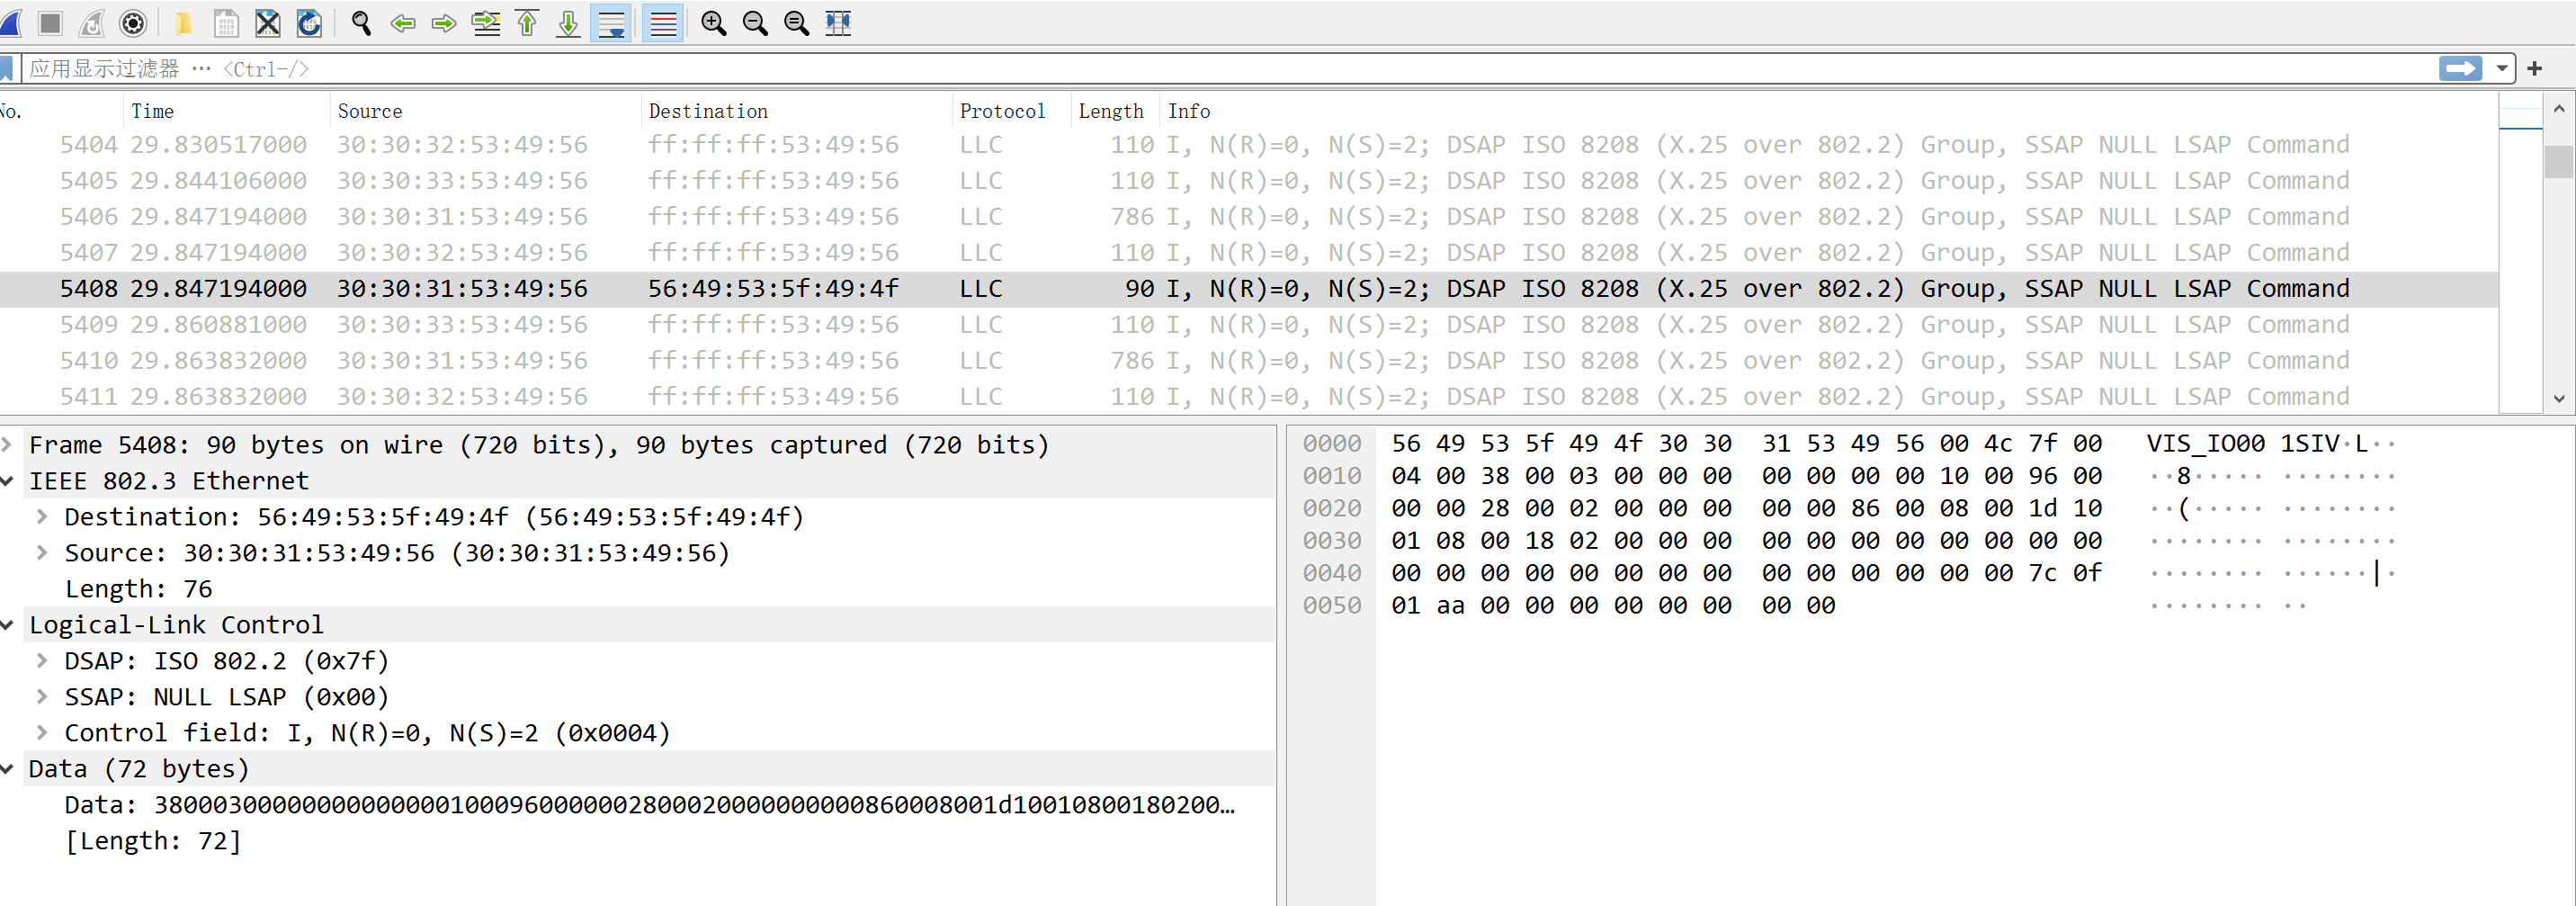
\includegraphics[width=\textwidth]{pictures/wireshark.png}
        \caption{WireShark抓包界面}
        \label{wireshark}
    \end{center}
\end{figure}
\section{WinPcap架构}
WinPcap(windows packet capture)是由意大利人Loris Degioanni在2000年提出并实现的一个架构,目的在于为Windows平台应用程序提供访问网络底层的能力\cite{winpcap1}。
传统socket通信中,两台主机之间通信,socket接收到的内容都是已经过网络协议栈处理的通信内容,并不会含有如数据帧头,IP头,TCP/UDP等内容。WinPcap功能在于独立于操作系统的网络协议栈而发送和接收数据帧,非常适合做网络协议分析、网络监控等工作\cite{winpcap2}。
\par
抓包系统必须绕过操作系统的协议栈来访问在网络上传输的数据帧,这就要求一部分运行在操作系统核心内部,直接与网卡驱动交互。Winpcap是针对Win平台上的抓包和网络分析的一个架构。它包括一个内核态的包过滤器,一个底层的动态链接库packet.dll和一个用户态的程序接口库wpcap.dll\cite{winpcap3}。
本系统中用其收取和发送数据链路层上的数据帧,帮助视景系统与仿真机交流。
\begin{figure}[h!]
    \begin{center}
        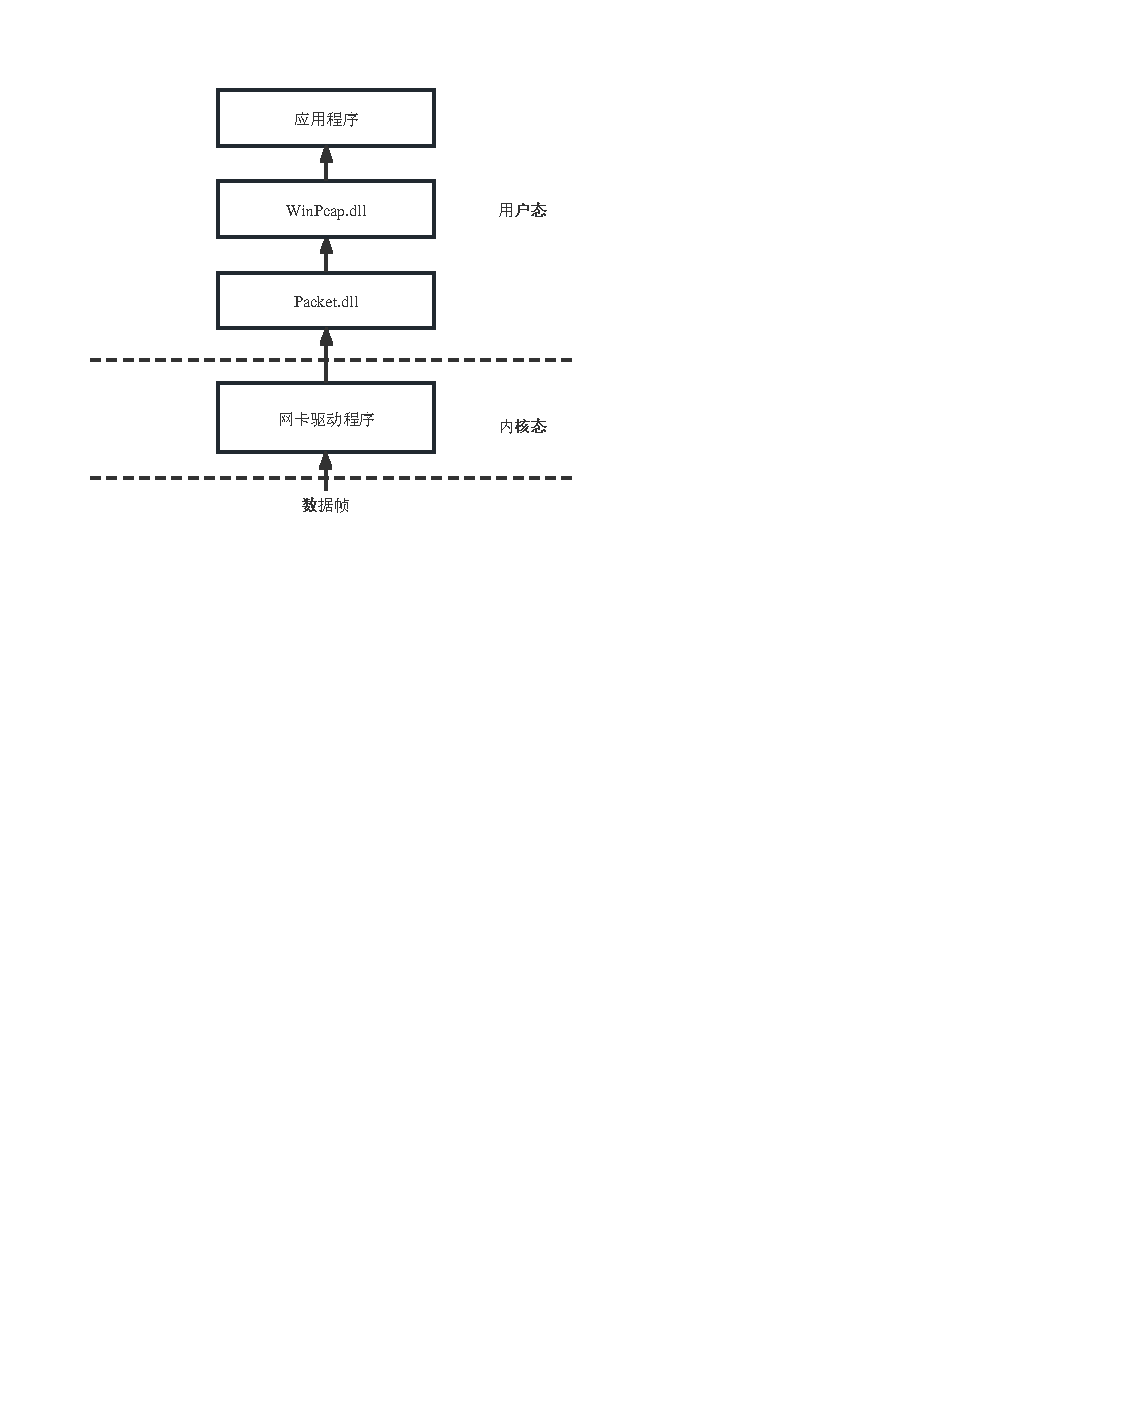
\includegraphics[width=0.6\textwidth]{pictures/winpcap.pdf}
        \caption{WinPcap结构}
        \label{wincapstruc}
    \end{center}
\end{figure}
\section{ProtoBuffer协议}
Protocol Buffer是Google提供的一种数据序列化协议,可用于通讯协议、数据存储等领域的语言无关、平台无关、可扩展的序列化结构数据格式\cite{Protobuf1}。它属于一种二进制协议,相比较文本协议如XML,JSON等在体积和封解包速度方面有巨大的优势\cite{Protobuf2},适合诸如本系统的实时渲染应用。
\par
ProtoBuffer序列化后消息紧凑得益于巧妙设计的编码方式。
首先其使用了Varint这种紧凑的表示数字的方法。它用一个或多个字节来表示一个数字,值越小的数字使用越少的字节数。这能减少用来表示数字的字节数。
Varint中的每个字节的最高位有特殊的含义,如果该位为1,表示后续的字节也是该数字的一部分,如果该位为0则结束,其他的7位都用来表示数字,因此小于128的数字都可以用一个字节表示,而不是统一为4个字节。
从统计的角度来说,一般不会所有的消息中的数字都是大数,大多情况下采用Varint可以用更少的字节数来表示数字信息。在进一步的优化中使用到了ZigZag编码,即用无符号数交错表示正数与负数,减少了负数的编码长度。
\par
其次ProtoBuffer对Key的定义为field\_number+wire\_type,field\_number表示该属性在结构中的编号,3位的wire\_type则指明了该属性的类型。
ProtoBuffer中共有6种wire\_type,如表\ref{pbtype}所示。
\begin{table}[h!]
    \begin{center}
        \caption{ProtoBuffer类型列表}
        \label{pbtype}
        \renewcommand\arraystretch{1.5}
        \begin{tabularx}{0.8\textwidth}{ 
            | >{\centering\arraybackslash\hsize=.5\hsize\linewidth=\hsize}X 
            | >{\centering\arraybackslash\hsize=.5\hsize\linewidth=\hsize}X 
            | >{\centering\arraybackslash\hsize=\hsize\linewidth=\hsize}X 
            | }
            \hline
            \textbf{ID} & \textbf{名称} & \textbf{包含类型}\\
            \hline
            0 & VARINT & int32, int64, uint32, uint64, sint32, sint64, bool, enum\\
            \hline
            1 & I64 & fixed64, sfixed64, double\\
            \hline
            2 & LEN & fixed64, sfixed64, double\\
            \hline
            3 & SGROUP & group start (deprecated)\\
            \hline
            4 & EGROUP & group end (deprecated)\\
            \hline
            5 & I32 & fixed32, sfixed32, float\\
            \hline
        \end{tabularx}
    \end{center}
\end{table}

\par
解包过程中XML需要从文件中读取出字符串,再转换为XML文档对象结构模型。之后再从XML文档对象结构模型中读取指定节点的字符串,最后再将这个字符串转换成指定类型的变量。其中的计算消耗无疑非常巨大。
ProtoBuffer在解包时只需要简单地将一个二进制序列,按照指定的格式读取到对应的结构体中就可以了。当然这也说明其必须要事先编写结构体文件给到接收方,否则无法正确解包。
\section{Tbuspp中间件}
Tbuspp是腾讯为完整解决游戏后台复杂与低延迟通讯需求而建立的服务网格中间件。
随着分布式架构越来越复杂和服务越拆越细,开发人员迫切的希望有一个统一的控制面维护和管理各项服务。边车模式有效分离了系统控制和业务逻辑,使开发人员专注业务逻辑\cite{tbus2}。
服务网格是用于处理服务间通信的基础设施层,服务可以插入其中的代理网格,代理作为边车注入到每个服务部署中\cite{tbus1}。服务间的调用通过代理实现,封装了其复杂性。
\par
Tbuspp的目标是构建功能完备的面向消息通讯中间件,能够完整解决全球同服部署模式下,游戏后台复杂与低延迟通讯需求,并能尽量降低开发与运维成本,做到简单易用。
其与Envoy等流行的开源服务网格组件有两点本质区别,第一是提供专用API供应用服务调用,与Envoy采用透明方式劫持应用服务的流量存在显著差异。
第二是基于SHM消息队列与应用服务交换消息,这点是针对游戏服务特殊的业务背景:游戏服务一般是有状态服务,希望在对服务快速重启更新的同时,保持游戏世界状态的连续性,因此往往需要将核心运行状态保存在SHM中,同时也基于SHM与边车交换消息,以便服务重启期间不间断消息收发。
本系统中使用Tbuspp作为虚拟仿真机与游戏引擎间进行TCP消息沟通的插件。
\section{Nagle算法}
在使用一些协议通讯时,如果每次只发送一个字节的有用信息,却要附带几十个字节的头部信息,这笔开销会增加拥塞情况的出现。
John Nagle就提出了一种通过减少需要通过网络发送包的数量来提高TCP/IP传输的效率\cite{nagle2},即Nagle算法。
Nagle算法核心是避免发送小的数据包,要求一个TCP连接上最多只能有一个未被确认的小分组,在该分组的确认到达之前不能发送其他的小分组。TCP会搜集这些小的分组,然后在之前小分组的确认到达后将刚才搜集的小分组合并发送出去。
\par
但Nagle算法也有弊端,对于实时性要求很高的交互上,我们不能使用Nagle算法\cite{nagle1}。
比如在网络游戏中,每一帧玩家的操作信息或状态改变并不会产生很大的包体,却需要及时的将状态同步到服务器中。此时若Nagle算法启用,部分信息将被延迟给到服务端,严重影响用户体验。
因此特别是在一些对时延要求较高的交互式操作环境中,必须禁用Nagle算法,让所有的小分组必须尽快发送出去。

\section{CrossEngine游戏引擎}
游戏引擎是打造出优秀游戏的核心因素之一,CrossEngine是腾讯为降低商业风险提升核心能力而自研的跨平台游戏引擎。其基础架构参考了ECS框架,
这是一种主要用于游戏引擎的软件开发架构,大体上由实体Entity、组件Component和系统System三部分构成\cite{ce1}。其中实体是对场景内需要逻辑控制的物体的抽象;组件代表被挂载于实体上的数据,一个实体可以搭载若干组件,相当于该实体被赋予了一系列属性;系统在此架构中承担了全部的逻辑代码,可以访问实体中的组件。
此架构突出了组合大于继承的理念,可以更加灵活的表示现实甚至想象出的概念。引擎中如内存分配、数学运算、资源管理等核心基本由C++编写,引擎编辑器主要由C\#开发。图\ref{ceeditor}展示了目前CrossEngine的编辑器界面。
\begin{figure}[h!]
    \begin{center}
        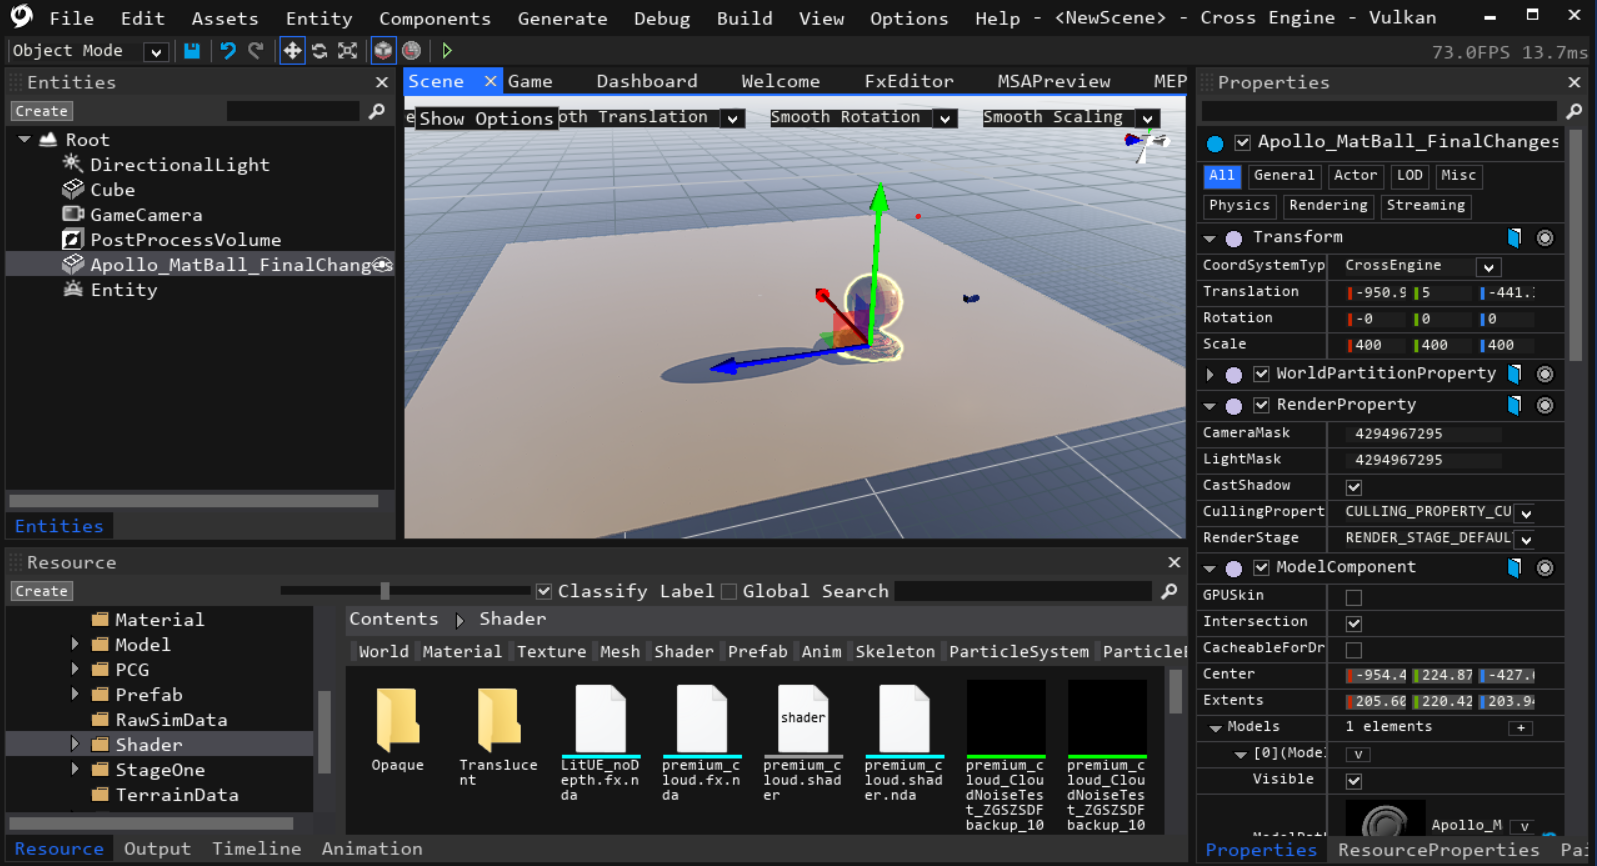
\includegraphics[width=0.9\textwidth]{pictures/crossengine.png}
        \caption{CrossEngine编辑器}
        \label{ceeditor}
    \end{center}
\end{figure}
\par
目前CrossEngine引擎已具备一定程度的生产实践能力。渲染方面目前已支持DX12、Vulkan、GLES3渲染后端,HDR-LinearSpace工作流内置基于物理的渲染;
功能系统方面具备基于PhysX的物理引擎,骨骼动画系统、粒子系统、脚本系统也基本完善。编辑器部分则是对标商业引擎主流设计,尽可能降低学习成本。
CrossEngine从最初的架构设计到三方基础库的选型都为Runtime尺寸做了许多工作,如表\ref{enginert}所示在该方面对比商业引擎有一定优势。在后续开发中也将坚持控制Runtime在较小的尺寸,以带来更多应用可能。
\begin{table}[h!]
    \begin{center}
        \caption{引擎Runtime比较}
        \label{enginert}
        \renewcommand\arraystretch{1.5}
        \begin{tabularx}{0.8\textwidth}{ 
            | >{\centering\arraybackslash\hsize=.5\hsize\linewidth=\hsize}X 
            | >{\centering\arraybackslash\hsize=.5\hsize\linewidth=\hsize}X 
            | }
            \hline
            \textbf{游戏引擎} & \textbf{Runtime体积} \\
            \hline
            CrossEngine & 2.2m \\
            \hline
            UnrealEngine4 & 40m+\\
            \hline
            Unity & 23m\\
            \hline
        \end{tabularx}
    \end{center}
\end{table}

% \section{Lua脚本}
% Lua 是一种用标准C语言编写而成的轻量级嵌入式脚本语言,其设计目的是为了嵌入应用程序中,从而根据不断变化的需求为应用程序提供灵活的扩展和定制功能\cite{Lua}。
% 不同于更广为人知的Python脚本,Lua诞生时的定位决定它并没有提供强大的库,所以Lua并不适合作为开发独立应用程序的语言,更多是调用宿主语言如C++中提供的核心方法以实现逻辑。因此Lua被广泛应用在游戏逻辑开发、openwrt系统中与宿主语言结合。
% 著名游戏《魔兽世界》中的客户端逻辑便是使用Lua编写。

% \par
% Lua作为解释性语言不需要编译过程,有更强的跨平台能力,且节省了开发过程中对于逻辑代码反复修改的编译时间,总之可以更灵活地应对各方面变动。本系统中用于观察系统效果和生成反馈信息的飞机飞行逻辑便是通过Lua脚本实现,其中调用如物体旋转、射线发射等游戏引擎中C++编写的方法,尽可能避免引擎核心的改动。

\section{航空坐标系及坐标系转换}
在模拟飞行中,涉及到位置和旋转的数据都是以某个坐标系为基础,常用坐标系有飞机自身坐标系、经纬高LLA坐标系、地心地固ECEF坐标系和北东天ENU坐标系。
其中只有LLA坐标系是以经度纬度海拔确认位置的坐标系,其余均为笛卡尔坐标系。
\begin{itemize}
    \item [(1)]
    飞机自身坐标系一般以驾驶舱位置为原点O,Z轴指向飞机下方,X轴指向飞机左侧,Y轴垂直于xOz平面指向飞机前方构成右手坐标系,如图\ref{crood1}所示。
    其作用为确定飞机上如起落架、各类灯的相对位置\cite{crood4}。
    \begin{figure}[h!]
        \begin{center}
            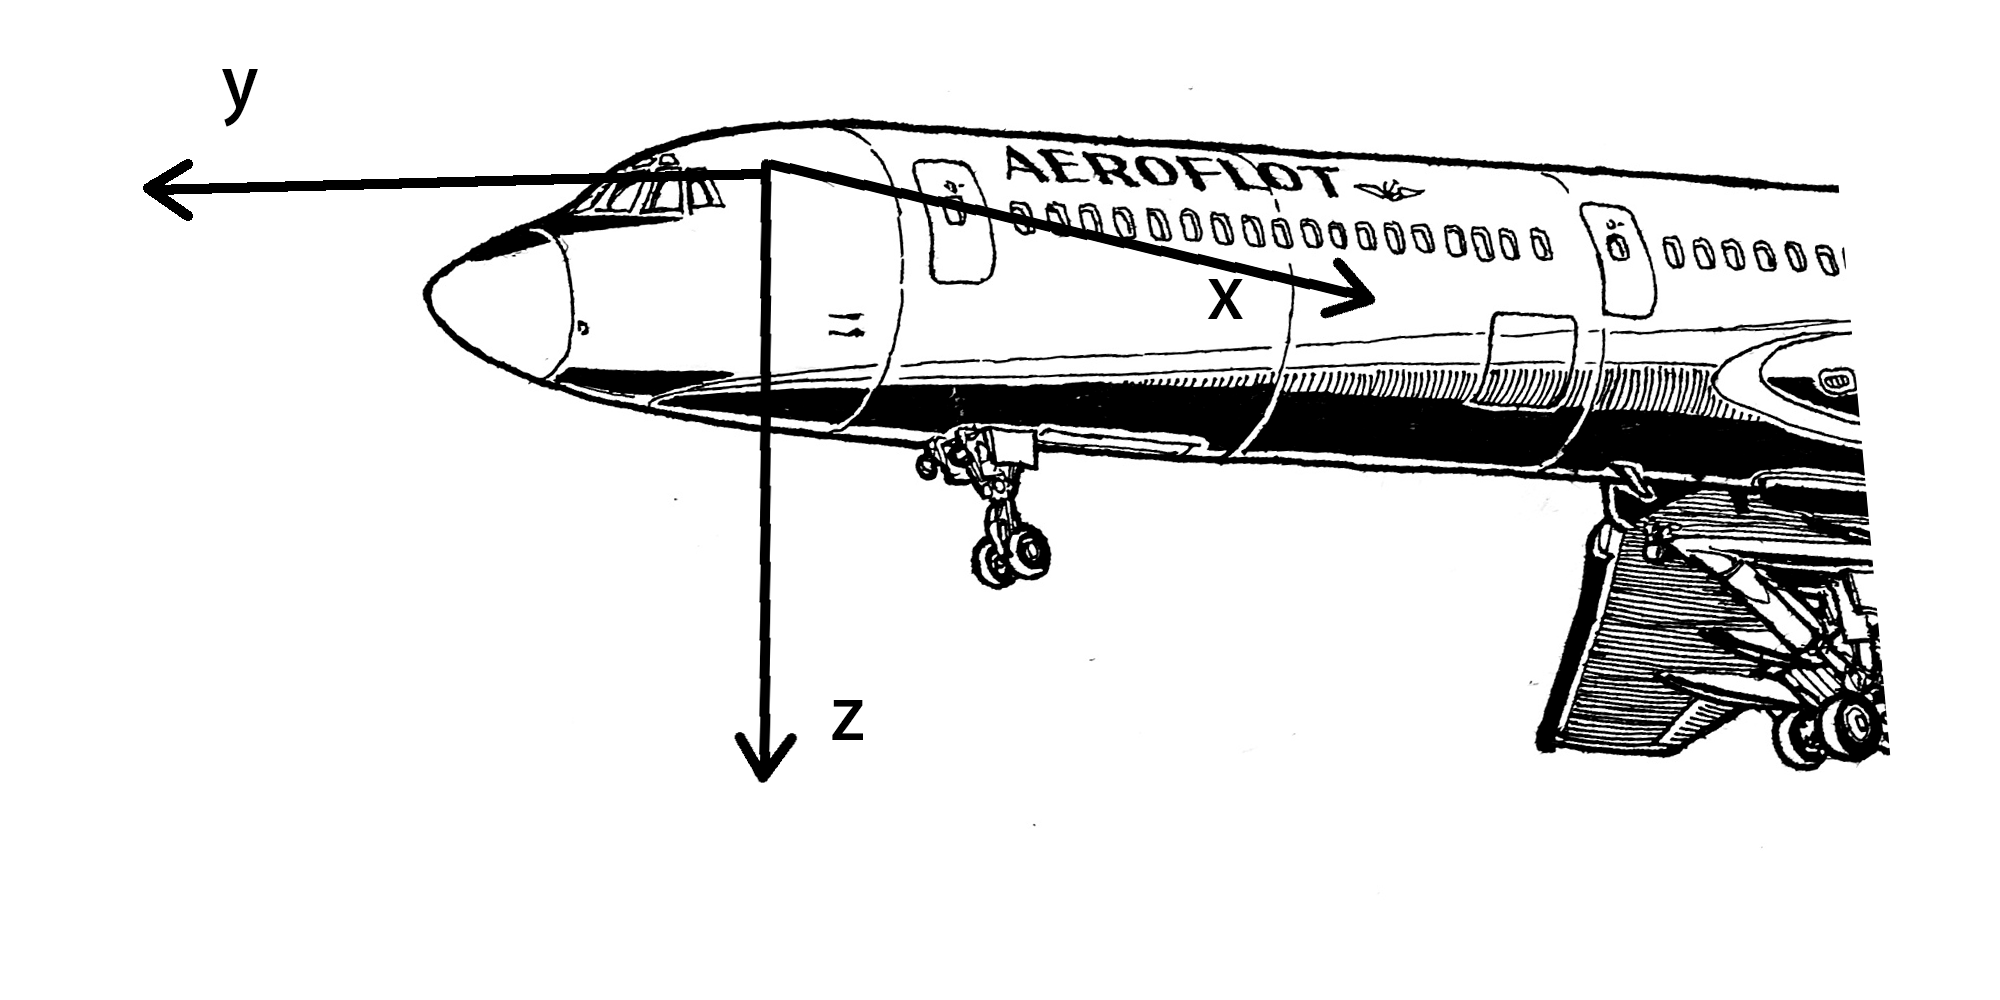
\includegraphics[width=0.8\textwidth]{pictures/plane.png}
            \caption{飞机自身坐标}
            \label{crood1}
        \end{center}
    \end{figure}
    \item [(2)]
    LLA坐标系是以经度纬度海拔来确定位置的球面坐标系。对地球而言经度的定义为本初子午线为0经度,向东增加。
    纬度的定义为椭球表面的法线与赤道面的夹角角度。海拔则是沿椭球表面法线方向距离平均海准面的距离。地球的形状则是以WGS-84为准,地球为长半轴6378137.0米,扁率1/298.257223563的椭球\cite{crood1}。
    在FFS中,仿真机给出的飞机位置信息便是经纬高的形式。
    \item [(3)]
    地心地固坐标系ECEF是一种以地心为原点的地固坐标系。原点O(0,0,0)为地球质心,Z轴与地轴平行指向北极点,X轴指向本初子午线与赤道的交点,Y轴垂直于xOz平面构成右手坐标系\cite{crood2}。
    在视景系统中需要以该坐标系作为世界坐标系,即所有物体的坐标最终都要转换到该坐标系下。
    \item [(4)]
    东北天ENU坐标系是以物体所在球面位置为原点,X轴指向东方,Y轴指向北方,Z轴垂直于xOy面指向天空构成的右手坐标系\cite{crood3}。
    在FFS中,每一帧下飞机的初始姿态便是在该坐标系下,且飞机的旋转是以偏航Yaw,俯仰Pitch,翻滚Roll的顺序完成。
    \begin{figure}[h!]
        \begin{center}
            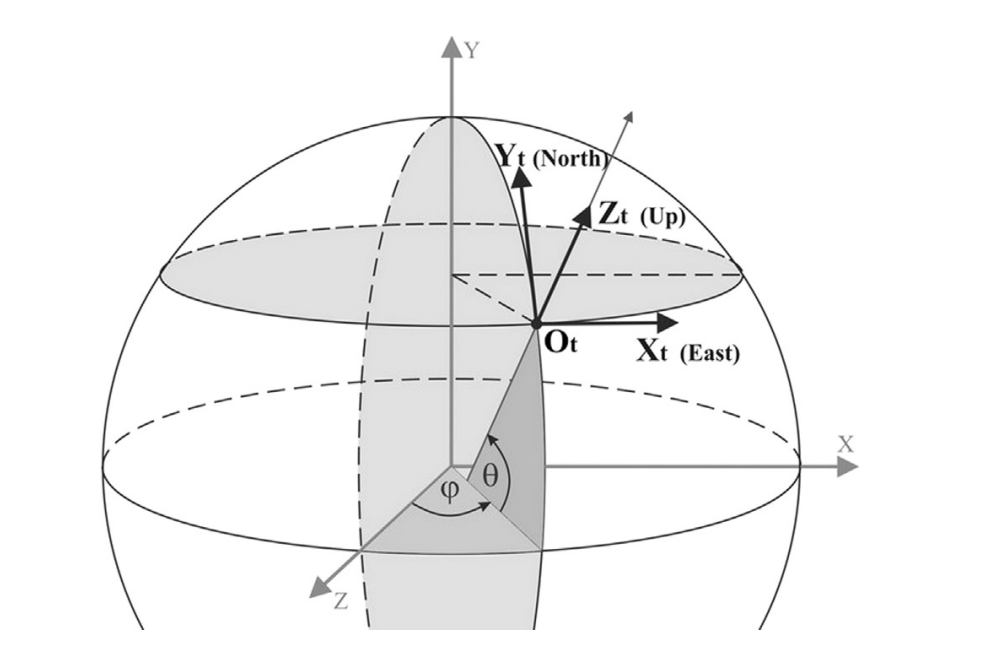
\includegraphics[width=0.8\textwidth]{pictures/coord.png}
            \caption{三类坐标系}
            \label{crood2}
        \end{center}
    \end{figure}
\end{itemize}
\par
以上是航空常用4种坐标系,在实际需求中必然涉及飞机的旋转以及坐标在不同坐标系下的变换。
向量的旋转和坐标的变换可以通过旋转矩阵表示\cite{rotate1}。最直观的旋转操作是按照固定坐标轴依次旋转,在三维空间中,按z轴旋转$\alpha$角度可以表示为如下形式。
旋转矩阵中的列向量为旋转后坐标系的坐标轴在旋转前的坐标系中的投影,自然互相正交且为单位向量,所以旋转矩阵为正交矩阵。旋转的逆变换可以直接使用转置矩阵作为逆矩阵。
~\\

\begin{math} 
    \begin{gathered}
        \begin{bmatrix} p_x' \\ p_y' \\ p_z'\end{bmatrix} 
        \quad 
        =
        \quad
        \begin{bmatrix} 
            cos(\alpha) & -sin(\alpha) & 0 \\
            sin(\alpha) & cos(\alpha) & 0 \\ 
            0 & 0 & 1
        \end{bmatrix}
        \quad
        \begin{bmatrix} p_x\\ p_y \\ p_z \end{bmatrix}
    \end{gathered}
\end{math}

~\\
\par
坐标系的转换也可视为旋转,特别要注意,上述公式中矩阵的意义是将点在旋转后的坐标系中的坐标,转换为旋转前的坐标系中的坐标。
此时将旋转矩阵中的列向量视作旋转后坐标轴在旋转前坐标轴上的投影,或者叫做方向余弦。

\par 
旋转在游戏引擎中都是通过四元数进行。四元数可以简单理解为一个任意旋转轴加旋转角度,对人类而言直观性会下降,但能够减少矩阵计算的复杂度,还可以方便的进行插值操作\cite{rotate2}。
使用欧拉角进行旋转时,中间的旋转取极端值不幸让某些坐标轴重合就会发生万向节死锁,
导致丢失一个方向上继续旋转的能力\cite{rotate3}。但在本项目中,仅就飞机的姿态而言是由仿真机给出的一个欧拉角直接确定,并不存在旋转叠加的问题,也就不会产生死锁。
\section{V-Sync垂直同步}
显示设备刷新一帧图像时,并不是一次性刷新整个图像,而是从上到下一行一行将图像绘制出来。
这个过程被称为逐行扫描,是目前显示设备最主要的成像方式。如果显示设备的刷新率为60Hz,意味着一秒钟可以通过该方式成像60次。
图像信息存放在显卡的缓冲区中,显卡会将渲染完毕的图像写入后缓冲区,与此同时前缓冲区中的图像会发送给显示设备。
后缓冲区中新鲜图像写入完成后,为减少拷贝过程,会直接将前缓冲区和后缓冲区的名字对调\cite{vsync1}。
问题在于如果前缓冲区中的图像刚部分发送给显示设备,两个缓冲区便进行交换,之后发送的便是下一帧的图像,在显示设备上产生画面撕裂。
图\ref{showtear}展示了产生画面撕裂的效果。
\begin{figure}[h!]
    \begin{center}
        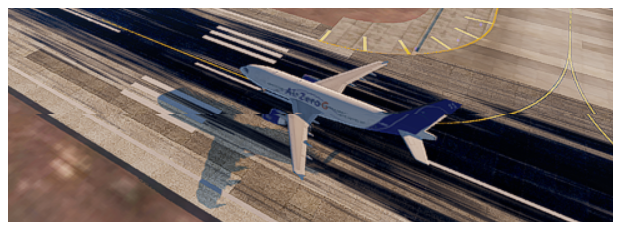
\includegraphics[width=\textwidth]{pictures/showtear.png}
        \caption{画面撕裂效果}
        \label{showtear}
    \end{center}
\end{figure}
\par
V-Sync垂直同步就是为了解决画面撕裂的问题。显示设备有自己的固定刷新率,在一次逐行扫描结束到下一次开始前会有小段间隙,
此时硬件会发出垂直同步脉冲保证前后缓冲可以在最佳的时间点交换\cite{vsync2},相当于限制了显卡的绘制频率。当然这只在显卡绘制频率大于显示设备刷新率时才有效果,否则依旧会有卡顿跳帧问题。
如图\ref{vsync}所示本系统中使用垂直同步来同步投影仪与逻辑帧和渲染帧的同步工作,避免画面撕裂。
\begin{figure}[h!]
    \begin{center}
        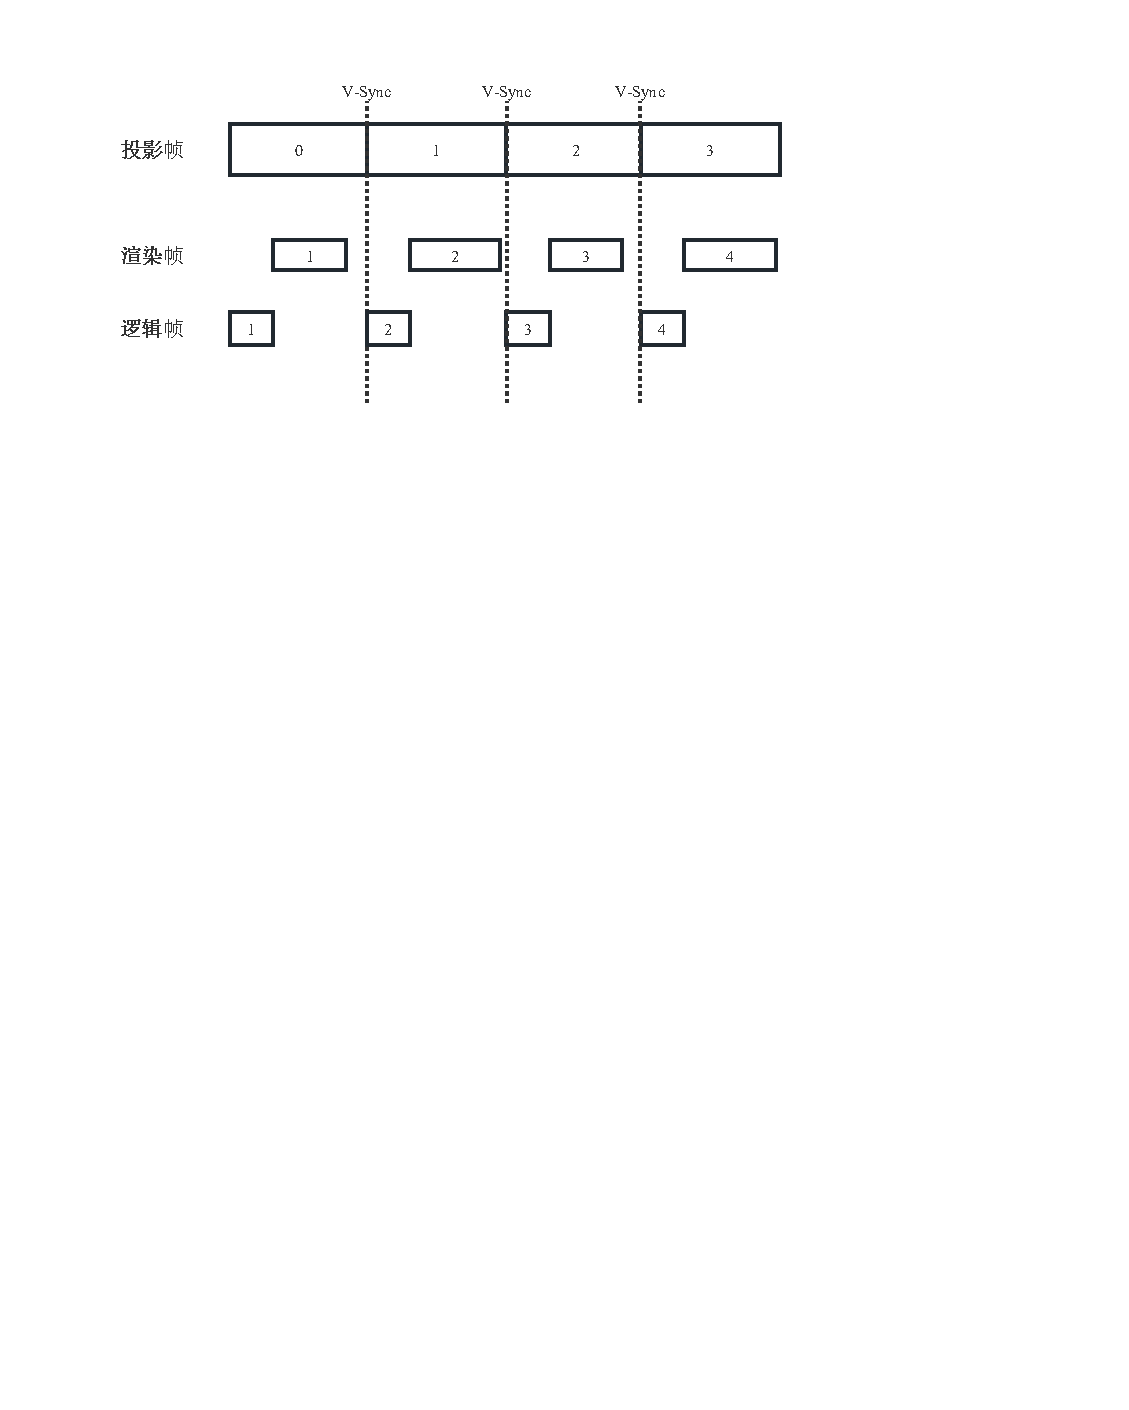
\includegraphics[width=0.8\textwidth]{pictures/vsync.pdf}
        \caption{垂直同步示意图}
        \label{vsync}
    \end{center}
\end{figure}
\section{本章小结}
本章介绍了视景系统中数据交换子系统开发中涉及的主要工具和技术。
在软件方面介绍了实现网络包捕获的WireShark工具;能够绕过操作系统网络协议栈的WinPcap架构;
负责TCP协议通信的Tbuspp;以及开发本视景系统的自研游戏引擎CrossEngine。
在技术方面介绍了具有高序列化与反序列化效率的ProtoBuffer协议;会造成小数据包发送延迟的Nagle算法;
飞行中用到的4种航空坐标系;以及V-Sync垂直同步技术。它们共同保证了视景系统中飞行画面的流畅与稳定。
